\section{Introduzione}
I raggi cosmici (RC) sono particelle elementari e nuclei  provenienti dall'universo che bombardano costantemente l'atmosfera terrestre. I RC sono solitamente classificati in due categorie: i \emph{primari}, ovvero le particelle cosmiche che incidono direttamente nell'alta atmosfera, tipicamente composti da protoni, particelle alpha e in parte minore da nuclei leggeri; i \emph{secondari}, prodotti dagli sciami adronici ed elettromagnetici generati dalle interazioni dei primari con l'atmosfera, e tipicamente composti da muoni, mesoni, adroni leggeri e nuclei.
\begin{figure}[h!]
\centering
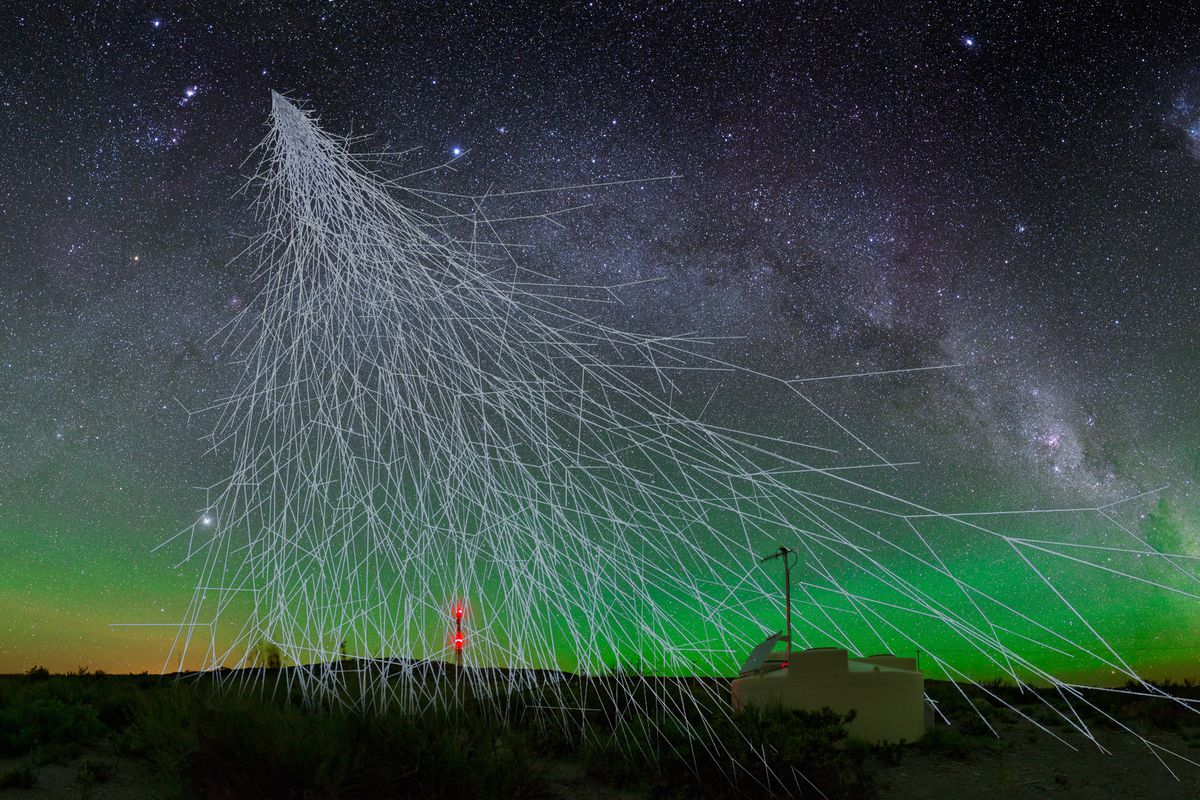
\includegraphics[width=0.45\textwidth]{pierre4HR.0.jpg}
\caption{Sciame prodotto da un raggio cosmico primario. \citep{immagine_cosmici}}
\end{figure}
 I RC sono noti fin dai primi decenni del '900 e la loro fisca è stata studiata approfonditamente nel corso degli anni. Ciononstante, alcuni aspetti non sono stati approfonditi, per cui risulta tutt'ora di grande interesse scientifico effettuare ricerca in questo campo. Le misure di interesse che vogliamo effettuare con il nostro esperimento sono: 
\begin{enumerate}
    \item \textbf{Misura di flusso verticale dei RC carichi in funzione dell'altitudine} - Il flusso verticale di raggi cosmici è atteso dipendere dalla quota: l'interazione adronica dei primari con l'atmosfera (Figura \ref{frammentazione primari}) dipende criticamente dalla densità del mezzo. Stimiamo che il massimo della produzione di secondari avvenga attorno ai 20km. Questa misura è di duplice interesse: correlazione con l'altitudine di formazione delle nuvole, rivelando un possibile ruolo dei RC nella loro formazione (esperimento CLOUD @CERN); stima dei danni da radiazione indotti sull'elettronica, importante per stimare i \textit{single event upset} nella strumentazione di missioni spaziali;
    \begin{figure}
        \centering
        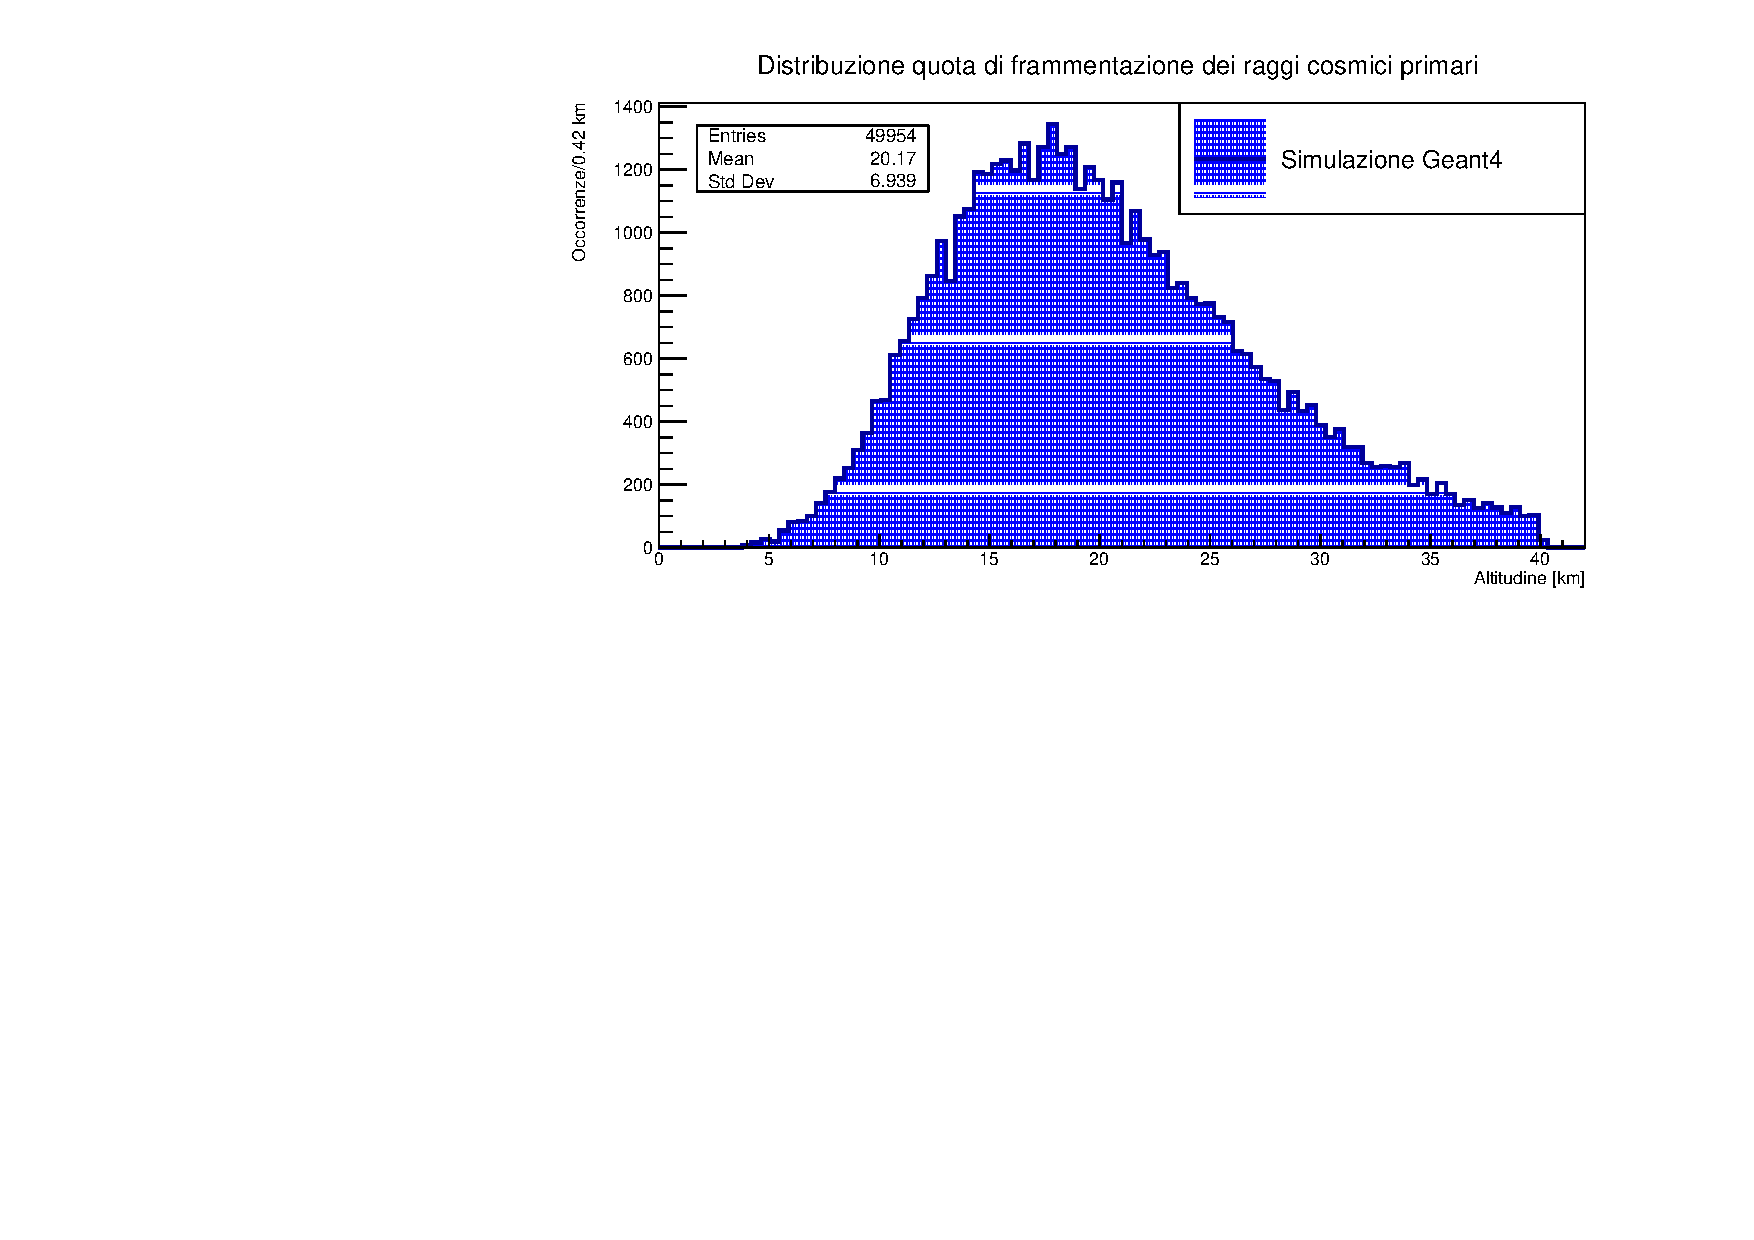
\includegraphics[width=0.5\textwidth]{Frammentazione_verticale.pdf}
        \caption{Simulazione GEANT4 della quota di frammentazione di un fascio di protoni energetici nell'atmosfera.}
        \label{frammentazione primari}
    \end{figure}
    
    \item \textbf{Misura di flusso orizzontale dei RC carichi in funzione dell'altitudine} - Ci si aspetta che la componente orizzontale dei RC sia fortemente soppressa, ma questo dipende dallo spessore trasverso di atmosfera attraversata, dunque dalla quota. Questa misura non è presente in letteratura e può apportare un contributo originale alla comprensione dei RC;
    \item \textbf{Misura del flusso di neutroni termici in funzione dell'altitudine} - I neutroni vengono prodotti in seguito a reazioni di spallazione nucleare tra la componente di raggi cosmici primari ed i nuclei di azoto e ossigeno. Lo spettro energetico risulta piccato per energie di $100\text{ KeV}$, come si osserva dalla Figura \ref{Neutroni}. Attraverso processi di scattering multiplo l'energia cinetica dei neutroni diminuisce, fino ad energie inferiori ad 1 $\text{eV}$. Neutroni con tale range di energie sono definiti termici. A queste energie diventano importanti fenomeni di assorbimento, in particolare si sottolinea il seguente:
\ce{n + ^{14}N -> ^{14}C + p}
, in cui da un nucleo di azoto si forma un particolare isotopo del carbonio. La reazione descritta regola la produzione e abbondanza relativa del carbonio-14 in natura. Dalla misura del flusso di neutroni termici possiamo ricavare il rate di produzione del $^{14}\text{C}$ in funzione della quota (Figura \ref{Carbonio}).
La misura è importante perché l'attività legata al carbonio-14 è uno dei metodi più diffusi di datazioni di reperti organici. 
\begin{figure}
    \centering
    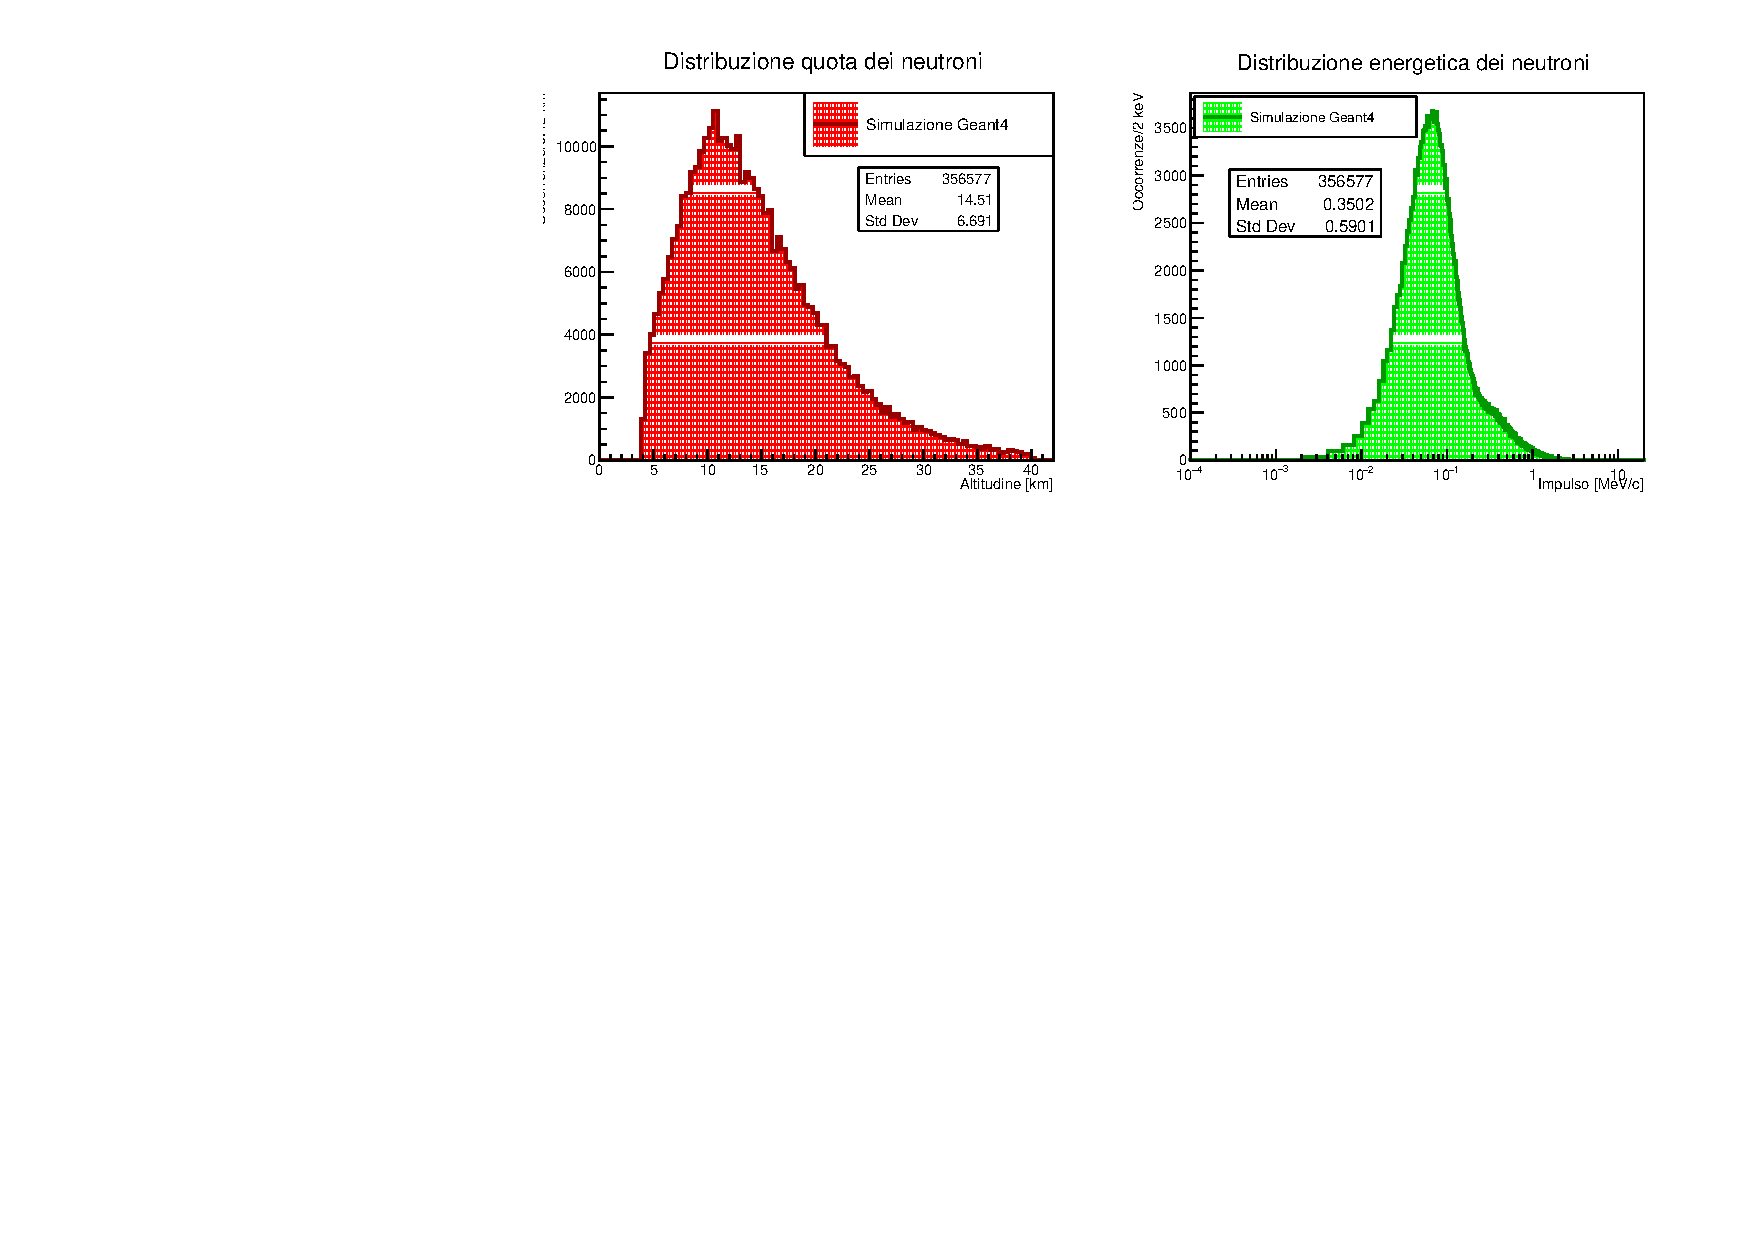
\includegraphics[scale=0.4]{Neutroni.pdf}
    \caption{Simulzione GEANT4 della quota e spettro energetico iniziale dei neutroni prodotti. Si noti come la distribuzione in quota segue quella dei protoni primari (Fig. \ref{frammentazione primari}).}
    \label{Neutroni}
\end{figure}
\begin{figure}
    \centering
    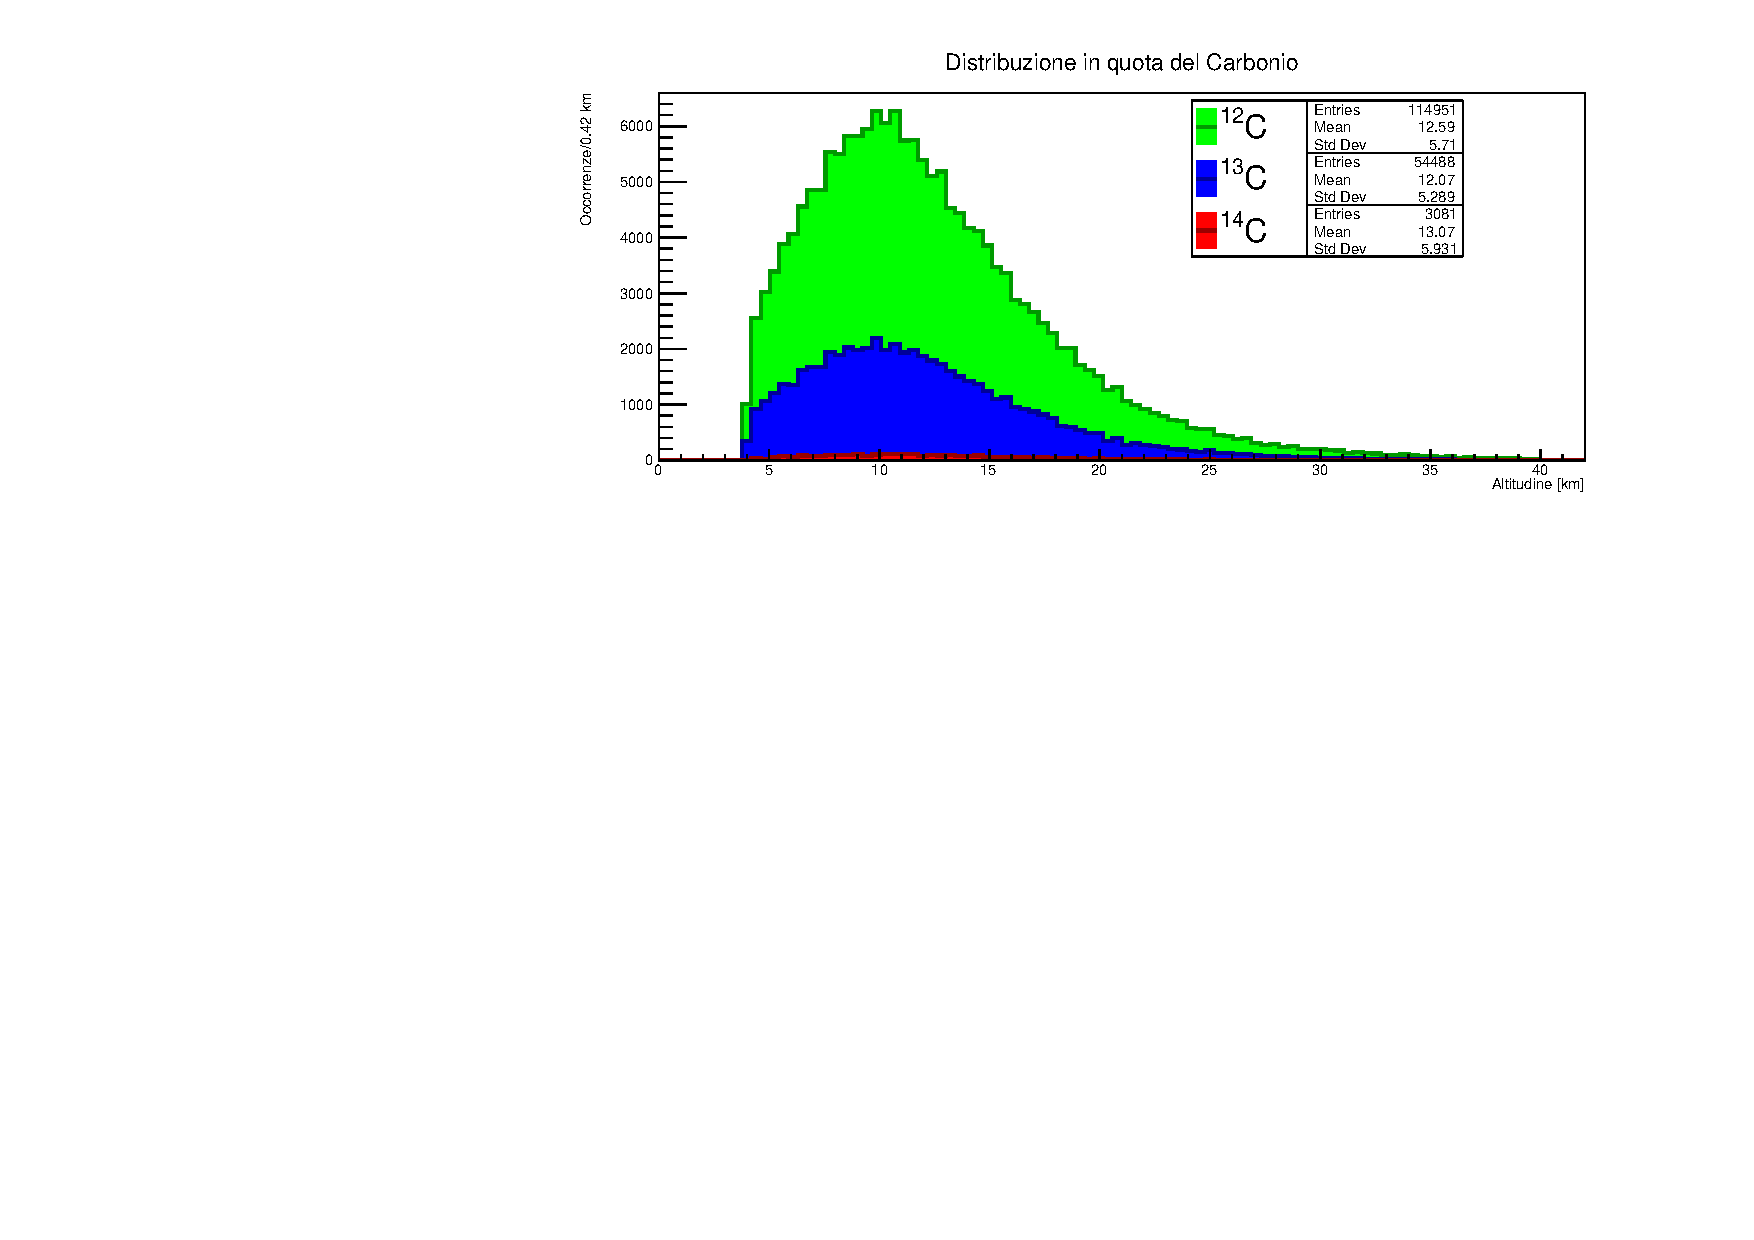
\includegraphics[scale=0.4]{Carbonio_verticale.pdf}
    \caption{Simulazione GEANT4 della distribuzione in quota degli isotopi del C prodotti dai RC primari.}
    \label{Carbonio}
\end{figure}

******** da inserire nella sezione rivelatori *****

Si propone una misura della componente termica del flusso di neutroni al variare della quota mediante l'impiego del dosimetro CT007-T (GammaGuard) 
\end{enumerate}
\bibliographystyle{plain}
\bibliography{references}
